\documentclass{article}
% !TEX root = Memoria.tex

\PassOptionsToPackage{numbers, compress}{article}

\usepackage[final]{nips_2017}

\usepackage[utf8]{inputenc} % allow utf-8 input
\usepackage[T1]{fontenc}    % use 8-bit T1 fonts
\usepackage{hyperref}       % hyperlinks
\usepackage{url}            % simple URL typesetting
\usepackage{booktabs}       % professional-quality tables
\usepackage{amsfonts}       % blackboard math symbols
\usepackage{amsmath}
\usepackage{nicefrac}       % compact symbols for 1/2, etc.
\usepackage{microtype}      % microtypography
\usepackage{subfiles}
\usepackage{xcolor}
\usepackage{multirow}
\usepackage{enumerate}
\usepackage{subfiles}
\usepackage{multirow}
\usepackage{graphicx}
\usepackage{subfiles}



\title{Práctica Final MAAA I}


\author{
	\AND
	Héctor Aldao Amoedo\\
	\texttt{hector.aldao@udc.es}\\  
	\And
	Laura Cabaleiro Pintos\\
	\texttt{laura.cabaleiro.pintos@udc.es}\\
	\And
	Donato José Cotardo Valcárcel \\
	\texttt{donato.cotardo@udc.es}\\
	\And
	José Romero Conde\\
	\texttt{j.rconde@udc.es}\\
	\And  
}

\begin{document}
	
	
	\maketitle
	
	\begin{abstract}
		
		resumen
		
	\end{abstract}
	
	\section{Introducción}
	
La preparación de datos es una etapa fundamental en el análisis de datos y el modelado predictivo, ya que garantiza la calidad de los datos y su compatibilidad con las técnicas utilizadas.

Para empezar, importamos el dataset de ejemplo 'Datos\_Práctica\_Evaluación\_1.csv' y lo cargamos en un DataFrame. Observamos el dataset, para luego extraer por pantalla el número de variables, instancias, individuos y las clases de salida que tiene este.

\begin{figure}[h]
    \centering
    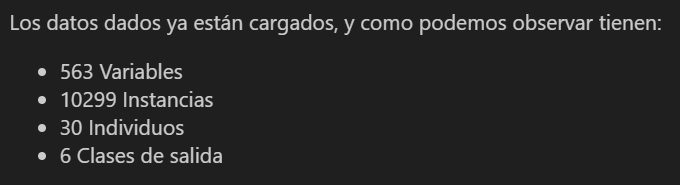
\includegraphics[width=0.75\linewidth]{images/datos.png}
    \caption{Número de cada dato pedido}
    \label{fig:enter-label}
\end{figure}

El análisis inicial identificó valores nulos en el 0.004656507546905259\% de las variables, entonces buscamos la solución para rellenar esos valores faltantes, porque es necesario preparar los datos antes del entrenamiento. Para las variables numéricas, los valores faltantes se imputaron utilizando la media, mientras que para las variables categóricas se utilizó la moda. Esto asegura que las distribuciones originales de los datos se mantengan intactas.

Posteriormente, normalizamos las columnas numéricas del DataFrame al rango [0,1], y luego convertimos variables categóricas en numéricas usando One-Hot Encoding, y así las columnas categóricas se convierten en columnas binarias. También validamos los datos para comprobar que se han transformado correctamente los valores.

La práctica nos pide segmentar el 10\% de los datos usando HoldOut, y luego comprobamos que no hay intersección entre los conjuntos, para comprobar que el conjunto de entrenamiento y HoldOut se ha formado correctamente. 

Luego realizamos un 5-Fold Cross-Validation a nivel de individuos, para que las instancias de un mismo individuo no se distribuyan entre conjunto de entrenamiento y test. Nos aseguramos que las instancias de un individuo estén presentes en un solo fold, con sus datos asociados, y vemos el número de participanetes únicos e instancias totales de cada fold.

Por último, realizamos una normalización MinMaxScaler a cada uno de los conjuntos resultantes para que asi cada uno tengo sus valores numéricos escalados al rango [0,1].
	\section{Blablabla}
	
	
	\section{Results} 
	
	
	\section{Conclusiones}
	
	conclusiones
	
	
	%\bibliography{deeplearn}
	\begin{thebibliography}{10}
		
		\bibitem{layernorm2016}
		Jimmy~Lei Ba, Jamie~Ryan Kiros, and Geoffrey~E Hinton.
		\newblock Layer normalization.
		\newblock {\em arXiv preprint arXiv:1607.06450}, 2016.
		ACL, August 2013.
		
	\end{thebibliography}
	
\end{document}
